\chapter{Introduction} \label{ch:introduction}

Many of the central questions in quantum information theory can be phrased as optimization problems. 
Given a quantum system, one may ask how much entanglement it contains, whether its correlations can be explained classically, which measurement best extracts the information encoded in it, or what resources are required to learn a desired property of a quantum signal. 
The mathematical structure of quantum theory makes semidefinite programming a particularly powerful tool for studying such questions. 
States are represented by positive semidefinite operators, measurements by collections of positive semidefinite operators summing to the identity, and many operational quantities can be written as linear functions optimized over these objects. 
This convex-optimization perspective has been central to many developments in quantum information.

However, the usefulness of this perspective is limited by two recurring obstacles. 
The first is computational hardness: some natural structural constraints, most notably separability, are NP-hard to test in general. 
The second is dimensionality: the Hilbert space of an $n$-qubit system has dimension $2^n$, so even optimization problems that are convex in principle may become computationally infeasible in practice. 
This thesis studies several problems where these barriers arise and develops methods that exploit hidden structure to reduce the effective dimension, enable hybrid quantum–classical computation, or provide provable guarantees for simpler measurement strategies.

The first part of the thesis concerns the \emph{separability problem}. 
Entanglement is one of the defining features of quantum theory and is a key resource in quantum information processing. 
A bipartite state is separable if it can be expressed as a convex combination of product states, and entangled otherwise. 
Determining whether a given state is separable is a fundamental problem, but it is NP-hard in general. 
Standard semidefinite programming relaxations, such as those based on the positive partial transpose condition or symmetric extensions, provide useful tests and hierarchies, but they still suffer from the exponential growth of the underlying Hilbert space. 
In this thesis, we introduce a hybrid algorithm that uses a quantum co-processor to reduce the effective dimension of optimization problems over separable states. 
A key feature of the method is that, even though it is heuristic in nature, it always produces a feasible separable state. 
Thus, the output is not merely a numerical bound, but an explicit valid candidate solution. 
We apply this approach to the problem of approximating the minimum separable energy of many-body Hamiltonians, which leads to a way of quantifying the entanglement present in their ground spaces. 
Numerically, this framework allows us to study systems with up to $28$ qubits, far beyond what a direct SDP formulation would permit.

The second part of the thesis studies several aspects of \emph{quantum state discrimination}. 
In its basic form, state discrimination is the task of identifying which state from a known ensemble was prepared. 
Since non-orthogonal quantum states cannot be perfectly distinguished, the goal is usually to optimize a chosen figure of merit, such as minimizing the probability of error or allowing inconclusive outcomes while avoiding mistakes. 
We first consider Helstrom’s general Bayes framework, in which the objective is specified by a reward or penalty assigned to each possible measurement outcome conditioned on each possible input state. 
This formulation unifies many discrimination tasks, including minimum-error discrimination, unambiguous discrimination, state exclusion, and more flexible objectives in which near-misses may receive partial credit.

From a practical viewpoint, we focus on the setting where the candidate states are not given as exponentially large classical vectors, but through their \emph{source code}: quantum circuits that prepare them. 
We show that the corresponding SDP can be reformulated entirely in terms of the Gram matrix of the candidate states. 
This reduces the SDP variable dimension from one depending on the Hilbert-space dimension $d$ to one depending on the number $N$ of candidate states and the number $L$ of possible guesses. 
Moreover, the Gram matrix can be constructed using quantum pre-processing procedures that estimate inner products directly from the preparation circuits. 
This yields a hybrid quantum–classical algorithm for Bayes-optimal quantum state discrimination. 
We apply the framework to quantum changepoint identification, including multiple-changepoint regimes and reward functions that account for approximate localization, and to quantum error type classification, where the reduction makes structured instances tractable for systems with hundreds of qubits.

We then turn to the exclusion variant of state discrimination. 
Whereas discrimination asks Bob to identify which state was sent, exclusion asks him to name a state that was not sent. 
This task is closely related to \emph{antidistinguishability} and can be viewed, in a precise sense, as optimizing the opposite objective from minimum-error discrimination. 
Motivated by the role of the \emph{pretty good measurement} as a simple and often effective approximation to the optimal discrimination measurement, we introduce the \emph{pretty bad measurement} as its analogue for exclusion. 
We prove that the pretty good and pretty bad measurements each satisfy a natural baseline guarantee: they perform at least as well as blind guessing in their respective objectives.

Finally, we study what happens when the most general measurement strategy is not physically available. 
Up to this point, the discrimination tasks allow joint measurements, which are the most general measurements one can perform on a collection of received quantum systems. 
Such measurements may require storing all systems coherently until the end of the protocol, which can be challenging experimentally. 
This motivates the question of whether joint measurements are always necessary, or whether simpler local strategies can still be optimal when the input has additional structure. 
We investigate this question for the task of evaluating Boolean functions from a sequence of quantum states. 
We compare two contrasting resource regimes. 
In the \emph{full-memory} setting, the entire finite sequence may be stored and an optimal joint measurement may be performed after all states have been received. 
In the \emph{memoryless} setting, neither quantum nor classical memory is available, and each state must be measured immediately using predetermined local measurements. 
We characterize which binary properties can still be learned optimally under these stringent constraints: a simple local greedy strategy is globally optimal precisely for affine Boolean functions, and more generally achieves at least the square of the optimal global success probability.

Together, the results of this thesis show that high-dimensional quantum optimization problems often contain structure that is invisible in their naive formulations. 
By identifying and exploiting this structure, one can reduce dimension, incorporate quantum subroutines into classical optimization pipelines, and obtain rigorous guarantees for simple measurement strategies. 
The thesis begins with a brief overview of the main topics, followed by the relevant background in linear algebra, quantum information, and semidefinite programming.

%%%%%%%%%%%%%%%%%%%%%%%%%%%%%%%%%%%%%%%%%%%%%%%%%%%%%%%%%%%%%%%%%%%%%%%%%%%%%%%%%%%%%%%%%%%%%%%%%%%%%%%%%%%%%%%%%%%%%%%%%%%%%%%%%%%
\section{Overview}
%%%%%%%%%%%%%%%%%%%%%%%%%%%%%%%%%%%%%%%%%%%%%%%%%%%%%%%%%%%%%%%%%%%%%%%%%%%%%%%%%%%%%%%%%%%%%%%%%%%%%%%%%%%%%%%%%%%%%%%%%%%%%%%%%%%

Quantum computing represents a paradigm shift in information processing, leveraging the fundamental principles of quantum mechanics, such as superposition and entanglement, to perform tasks that are beyond the reach of classical computation.
A primary objective has been to characterize the resources required to achieve a speedup over classical computation, which is referred to as ``quantum speedups''.
Shor's algorithm for integer factorization is a common example where using a quantum computer, one can achieve an exponential speedup over the best known classical algorithm.
Another example is Grover's algorithm which provides a quadratic speedup for an unstructured search problem compared to the best possible classical algorithm.

Semidefinite programming (SDP) has become an indispensable tool in quantum information theory, as evidenced by several seminal results. 
In particular, \cite{jain2011qip} used the matrix multiplicative weights update method to approximate the optimal value of an SDP to prove that the complexity classes QIP (quantum interactive proof systems) and PSPACE (problems that can be decided when the amount of space available is polynomial) are equivalent. 
More recently, \cite{ji2021mip} employed the NPA hierarchy to show that multi-prover interactive proofs with entangled quantum provers (MIP*) can decide all recursively enumerable (RE) languages. 
Together, these works exemplify how semidefinite programming and its associated hierarchies can resolve deep structural questions in quantum information.

While these results highlight the power of semidefinite programming in resolving deep questions in computational complexity, this thesis employs SDPs as both a theoretical framework and a practical computational tool to investigate two specific areas of quantum information: the characterization of entanglement and the optimal discrimination of quantum states. 
The remainder of this section outline the specific problems addressed in this work, beginning with the challenges of identifying entanglement in bipartite systems.

\subsection{Separability problem}

Entanglement is at the heart of many quantum problems and applications~\cite{horodecki2009quantum}.   
Even though it has been studied for a long time now, entanglement is still a mysterious resource and understanding its power and limitations is an interesting area of research.  

Given a quantum state, determining whether it is entangled or separable (i.e., not entangled) is called the \emph{separability problem}.
This problem is known to be NP-hard in general~\cite{gurvits2004classical,gharibian2010strong}. 
In the general case one could consider the entanglement of a multipartite state, but we restrict our attention to the bipartite case.
%If $\dim(\A) \cdot \dim(\B) \leq 6$, then it turns out that this problem has a finite-sized semidefinite programming formulation~\cite{horodecki1996necessary} while for all other cases, it was shown that no finite-sized semidefinite program exists~\cite{fawzi2021set}. 

To tackle this, several SDP relaxations exist that provide necessary but not necessarily sufficient conditions for separability. 
The most prominent one is the Peres-Horodecki criterion, or the \emph{Positive Partial Transpose} (PPT) condition, which states that any separable state must remain positive semidefinite under the partial transpose operation \cite{peres1996separability, horodecki1996necessary}. 
Although the PPT condition is both necessary and sufficient for low-dimensional systems (specifically $2 \times 2$ and $2 \times 3$), it is only sufficient in higher dimensions. 
To address this, more sophisticated methods such as the realignment criterion \cite{chen2003matrix, rudolph2005further} and the Doherty-Parrilo-Spedalieri (DPS) hierarchy of symmetric extensions \cite{doherty2002SymExt} have been introduced. 
The latter utilizes a hierarchy of SDPs that provides an increasingly tight outer approximation of the set of separable states, converging to it in the limit of infinite extensions.

Despite having a diverse array of applications~\cite{ioannou2007computational, brandao2011quasipolynomial, gharibian2013qma, chailloux2012complexity, hayden2013two, li2014quantum, consiglio2022variational, jeronimo2023power}, 
this problem is hard for two key reasons.   
For one, even if one were to exhibit a purported optimal solution, verifying its separability could be (NP) hard. 
Also, it suffers from the curse of dimensionality. 
In particular, when the two systems are $n$-qubit spaces, we are dealing with a problem that %$\tau \in \SepD$ 
has dimension $2^{2n}$ which renders many numerical computations infeasible. 

In Chapter~\ref{ch:Sep}, we address both of these issues by combining semidefinite programming techniques with quantum heuristics. 
Firstly, by using semidefinite programming-based algorithms, one can solve small instances (i.e., when the dimensions of the two systems are small) with reasonable levels of success. 
Secondly, we introduce a heuristic algorithm to  reduce the dimension of the optimization problem. 
We discuss when this pre-processing step can be run on a quantum co-processor, thereby alleviating the curse of dimensionality. 
In a sense, we do not need to perform any vector-represented calculations, the interactions are done on a quantum mechanical level and the desired quantities can be inferred from measurement statistics. 
We combine both of these methods, allowing us to optimize over separable states of large dimensions. 

We note that even though our algorithm is heuristics-based, it maintains an important feature which is that it always returns a feasible solution.\footnote{Interestingly, even if the quantum processing part of our method is noisy, it still returns a feasible solution.} 
Thus, in the event that our algorithm does not perform well,\footnote{Due to assumed complexity theoretical barriers (P $\neq$ NP), this is likely the case eventually for any such algorithm.} it still exhibits a feasible solution which could still be of value depending on the application. 

As an application, we approximate the separable state that has the greatest energy with respect to a fixed Hamiltonian, whose energy we call the \emph{separable ground energy}.\footnote{Note that since we are maximizing throughout the discussions in this work, we think of the largest eigenvalue as the ground energy. 
This convention is without loss of generality since one can replace the Hamiltonian $H$ with $-H$ if one prefers to minimize.} 
We show that this approximation can be used to characterize the amount of entanglement in the groundspace of the Hamiltonian. 
We give a full study of our algorithm for the case of the one-dimensional Ising Hamiltonian with numerics for up to $28$ qubits.

%%%%%%%%%%%%%%%%%%%%%%%%%%%%%%%%%%%%%%%%%%%%%%%%%%%%%%%%%%%%%%%%%%%%%%%%%%%%%%%%%%%%%%%%%%%%%%%%%%%%%%%%%%%%%%%%%%%%%%%%%%%%%%%%%%%

\subsection{Quantum state discrimination}

Quantum state discrimination is a central task in quantum information processing.
Quantum key distribution~\cite{ko2018advanced}, two-party cryptography~\cite{aharonov2000quantum, van2002unambiguous, cabello2000quantum, ambainis2001new, sikora2017simple}, the hidden subgroup problem~\cite{hayashi2008quantum}, quantum algorithms~\cite{radhakrishnan2009random, hayashi2008quantum}, and dimension witnessing~\cite{strubi2013measuring}, among many others, can all be formulated in terms of this problem, which can be described as the following two-party game.
%The quantum state discrimination problem can be phrased as a game between Alice and Bob. 
Alice has a finite set of quantum states $\{ \rho_1, \ldots, \rho_n \}$ and a fixed probability distribution $\{ p_1, \ldots, p_n \}$, both of which are known to Bob. 
Alice then samples $i$ with probability $p_i$, and prepares and sends $\rho_i$ to Bob. 
Bob wins the game if he correctly identifies the state by sending the correct index, $i$, back to Alice. 
This game is illustrated in Fig.~\ref{fig:ch4_PBM-fig1}.  
\begin{figure}[h] 
    \centering
    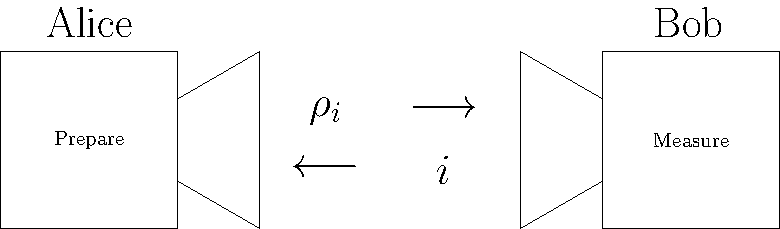
\includegraphics[scale=0.75]{figs/ch4_PBM/qsd_figure.pdf}
    \caption{Alice prepares $\rho_i \in \{ \rho_1, \ldots, \rho_n \}$ and sends it to Bob. 
    Bob wins the game if he correctly identifies the index $i$.}
    \label{fig:ch4_PBM-fig1}
\end{figure}

%Alice chooses a state from a fixed set of states and sends it to Bob who wishes to identify the state. 
%Here we assume that both Alice and Bob know the set of states and the a priori probabilities before the game commences.

For Bob to determine his state perfectly, the necessary and sufficient condition is that the states in the set must be pairwise orthogonal.
However this need not be the case and, in such circumstances, Bob may wish to optimize some desired figure of merit.
%, e.g., the average probability of correctly identifying the state.
This problem has fueled nearly five decades of work \cite{helstrom1969quantum}, producing extensive catalogs of state ensembles and their optimal discrimination probabilities \cite{sun2001optimum,sugimoto2010complete,herzog2004minimum,herzog2005optimum,herzog2015optimal}. 

Two figures of merit have received particular attention: minimum-error discrimination \cite{bae2013structure} where Bob outputs a guess with the goal of minimizing the overall probability of error, and unambiguous discrimination \cite{ivanovic1987differentiate, dieks1988overlap, peres1988differentiate} which forbids incorrect guesses altogether at the cost of allowing inconclusive outcomes. 
Closed-form solutions are known only for some particular ensembles in both of these paradigms \cite{jaeger1995optimal,barnett2009quantum}. 
However, the optimal discrimination probability for an arbitrary ensemble can be efficiently obtained using an SDP \cite{eldar2003designing,eldar2003semidefinite}.

Several other figures of merit exist depending on the desired application.
%For example, Bob may wish to only guess when he knows he will be correct, called unambiguous state discrimination.
Each figure of merit could correspond to adopting a different strategy which would in turn lead to different behavior.  
We discuss several variants in this thesis and refer the interested reader to the following reviews~\cite{chefles1998quantum, chefles2000quantum, bergou2004discrimination, bergou2007quantum, barnett2009quantum, bergou2010discrimination, Bae_2015}. 

In Chapter~\ref{ch:QSD} we consider the general Bayes framework, as introduced by Helstrom, for state discrimination when, instead of a classical description of the candidate states, one has access to their \emph{source code}: the quantum circuit that perpared them.
Observe that if we have $N$ such states each of dimension $d$ with $L$ possible guesses, then we are solving an SDP of dimension $d L$.
We first show how this problem can be reduced to solving an SDP of dimension $NL$, and then introduce a quantum pre-processing procedure which efficiently constructs the reduced SDP from the source code, enabling our method to operate directly on quantum data.
We consider two applications.
First, we characterize the optimal identifications for quantum changepoint problems under several reward structures, including multiple changepoint settings that were previously computationally inaccessible.
Second, we consider a quantum error classification problem and show how our reduction makes it tractable for systems of hundreds of qubits.

\begin{comment}
Preparing and measuring quantum states are the two pillars of quantum computing. 
As an example, quantum state tomography is the task of identifying which quantum state a device is preparing given (many) samples~\cite{christandl2012reliable, torlai2018neural, gross2010quantum, qi2013quantum, ahmed2021quantum, mahler2013adaptive, schwemmer2015systematic}
which has been experimentally tested~\cite{cramer2010efficient, stricker2022experimental, rambach2021robust, rippe2008experimental, mallet2011quantum}. 
In other words, one wishes to find the best measurement(s) to perform in order to learn the state with the fewest number of samples.

Another task central to quantum computing is the \emph{quantum state discrimination problem} where one is tasked with identifying which state they have been given \emph{from a fixed set of quantum states}. 
This is a naturally occurring setting which has been studied in the context of quantum algorithms~\cite{radhakrishnan2009random, hayashi2006quantum}, quantum cryptography~\cite{van2002unambiguous, cabello2000quantum, ambainis2001new, sikora2017simple}, quantum machine learning~\cite{sentis2016quantum, sentis2017exact}, among many others (see~\cite{Bae_2015} for a survey).
\end{comment}

\subsubsection{Pretty good measurement}

Consider the case where Bob wishes to maximize the average probability of correctly identifying the state. 
Suppose he measures with the measurements $\{M_1, \ldots, M_N\}$ and on outcome $j$ he guesses the state was $\rho_j$. 
Then, given state $\rho_j$, he guesses ``I think the state is $\rho_i$'' with probability 
$\inner{M_i}{\rho_j}$.  
In this case, he wins the game with probability 
%\begin{equation} 
$\sum_{i=1}^N p_i \inner{M_i}{\rho_i}$.  
%\end{equation} 
If Bob wishes to maximize this probability, then he is tasked with finding the best measurements $\{M_1, \dots, M_N\}$, known as the \emph{minimum error} measurement, and we define the best probability for Bob as 
\begin{equation}
    \label{eq:ch4_PBM-P_best} 
    \Pbest = \text{maximize} \; \sum_{i=1}^N p_i \inner{M_i}{\rho_i}.
\end{equation} 

Given a problem instance, one can numerically solve for the best measurements using semidefinite programming~\cite{cvx}. 
Unfortunately, characterizing such POVMs is a difficult task known only to be possible in special cases, e.g., for $N=2$ the case of two states~\cite{helstrom1969quantum}, for $N$ arbitrary qubit states given with equal \emph{a priori} probabilities~\cite{deconinck2010qubit}, for geometrically uniform states~\cite{eldar2004optimal}, and mirror symmetric states~\cite{andersson2002minimum}.  
Therefore, it is important to find generic classes of measurements which have a simple form and \emph{approximate} $\Pbest$.

The pretty good measurement (PGM), first discussed in~\cite{belavkin1975optimaldist, belavkin1975optimal, hughston1993complete}, is a way to approximate the best possible measurement. 
The PGM is known to be optimal in certain cases, some nice examples being for the hidden subgroup problem~\cite{bacon2005optimal, moore2005distinguishing}, for the quantum change point problem~\cite{sentis2016quantum}, and in port-based teleportation~\cite{leditzky2022optimality}.  
Generally speaking, for problems with a large amount of symmetry, the PGM seems to perform well. 

\subsubsection{Quantum state exclusion}

The quantum state \emph{exclusion} problem is similar to quantum state discrimination except that Bob wishes to guess a state \emph{which was not sent}. 
For example, if Alice sends $\rho_1$ to Bob and Bob responds with ``Alice, you did not send $\rho_3$'' then he would win the game in that case. 
The work in \cite{bandyopadhyay2014conclusive} studies this task in detail and its relationship to the PBR game~\cite{pusey2012reality}. 
Quantum state exclusion is illustrated in Fig.~\ref{fig:ch4_PBM-fig2}.  
\begin{figure}[h] 
    \centering
    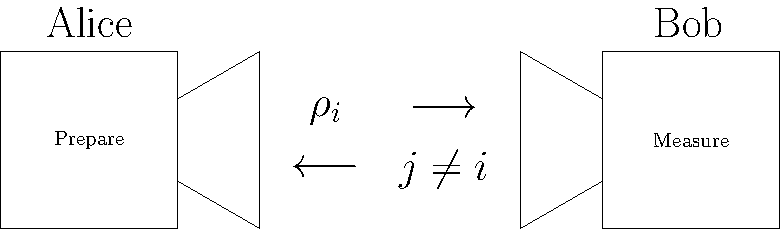
\includegraphics[scale=0.75]{figs/ch4_PBM/qse_figure.pdf}
    \caption{Alice prepares $\rho_i \in \{ \rho_1, \ldots, \rho_n \}$ and sends it to Bob. 
    Bob wins the game if he correctly \emph{excludes} an index $j \neq i$.}
    \label{fig:ch4_PBM-fig2}
\end{figure} 

Unlike quantum state discrimination, it is much more difficult to determine when Bob has a perfect strategy to perfectly win this game, i.e., when he can exclude a state without error. 
If this is the case, we say that the states are \emph{antidistinguishable} which has been the topic of recent research~\cite{havlivcek2020simple, russo2023inner, leifer2020noncontextuality, mishra2023optimal, uola2020all, johnston2023tight}. 

If Bob wishes to find the measurement which best excludes a state, he wishes to minimize the probability of making an incorrect guess.
More precisely, if Bob measures $\rho_i$ with the measurements $\{M_1, \ldots, M_N\}$, he makes an \emph{incorrect guess} with probability $\inner{M_i}{\rho_i}$.  
Thus, he wishes to \emph{minimize} 
%\begin{equation} 
$\sum_{i=1}^N p_i \inner{M_i}{\rho_i}$.  
%\end{equation} 

Notice that this is the exact opposite of what he wishes to do in the quantum state discrimination problem where he wants to maximize this quantity, see Eq.~\eqref{eq:ch4_PBM-P_best}. 
Thus, if Bob wants to exclude a state, his best measurement is also the \emph{worst} measurement for discrimination. 
Therefore, we define 
\begin{equation}
    \label{eq:ch4_PBM-P_worst}
    \Pworst = \text{minimize} \; \sum_{i=1}^N p_i \inner{M_i}{\rho_i}. 
\end{equation}

It is worth noting that the viewpoint of Bob trying to lose the quantum state discrimination game is interesting in its own right. 
Indeed, Bob cannot always lose this game with certainty, even if he wants to, and understanding when this is the case, and more generally, understanding the above quantity gives insights into the very nature of quantum information.

Chapter~\ref{ch:PBM} focuses on constructing an analogue of the PGM for approximating $\Pworst$.

\subsubsection{Memoryless regime}

Suppose now that Bob knows two quantum states $\ket{\psi}$ and $\ket{\phi}$, and he is promised that every one of the candidate states is a sequence of the form
\begin{equation}
    \ket{\psi} \otimes \ket{\phi} \otimes \ket{\psi} \otimes \cdots \otimes \ket{\psi}.
\end{equation}
While each position is known to be either $\ket{\psi}$ or $\ket{\phi}$, the identity of each state is unknown.
Can Bob determine whether the number of $\ket{\psi}$ states exceeds the number of $\ket{\phi}$ states, or whether the total number of $\ket{\psi}$ states is even?
These examples highlight a basic task: learning coarse-grained properties of a quantum sequence without necessarily determining the sequence itself.

We study this problem in two contrasting resource regimes as illustrated in Figure~\ref{fig:ch1_global_vs_greedy}.
In the \emph{full-memory} setting the entire (finite) sequence may be stored so that an optimal joint measurement can be performed upon receiving all of the states.
In the \emph{memoryless} setting, neither quantum nor classical memory is available and each state must be measured immediately, using only predetermined local measurements.
This work investigates which binary properties (properties which can be either true or false) can still be learned optimally under such stringent memory constraints.

\begin{figure}[h]
    \centering
    \begin{subfigure}[b]{0.495\textwidth}
        \centering
        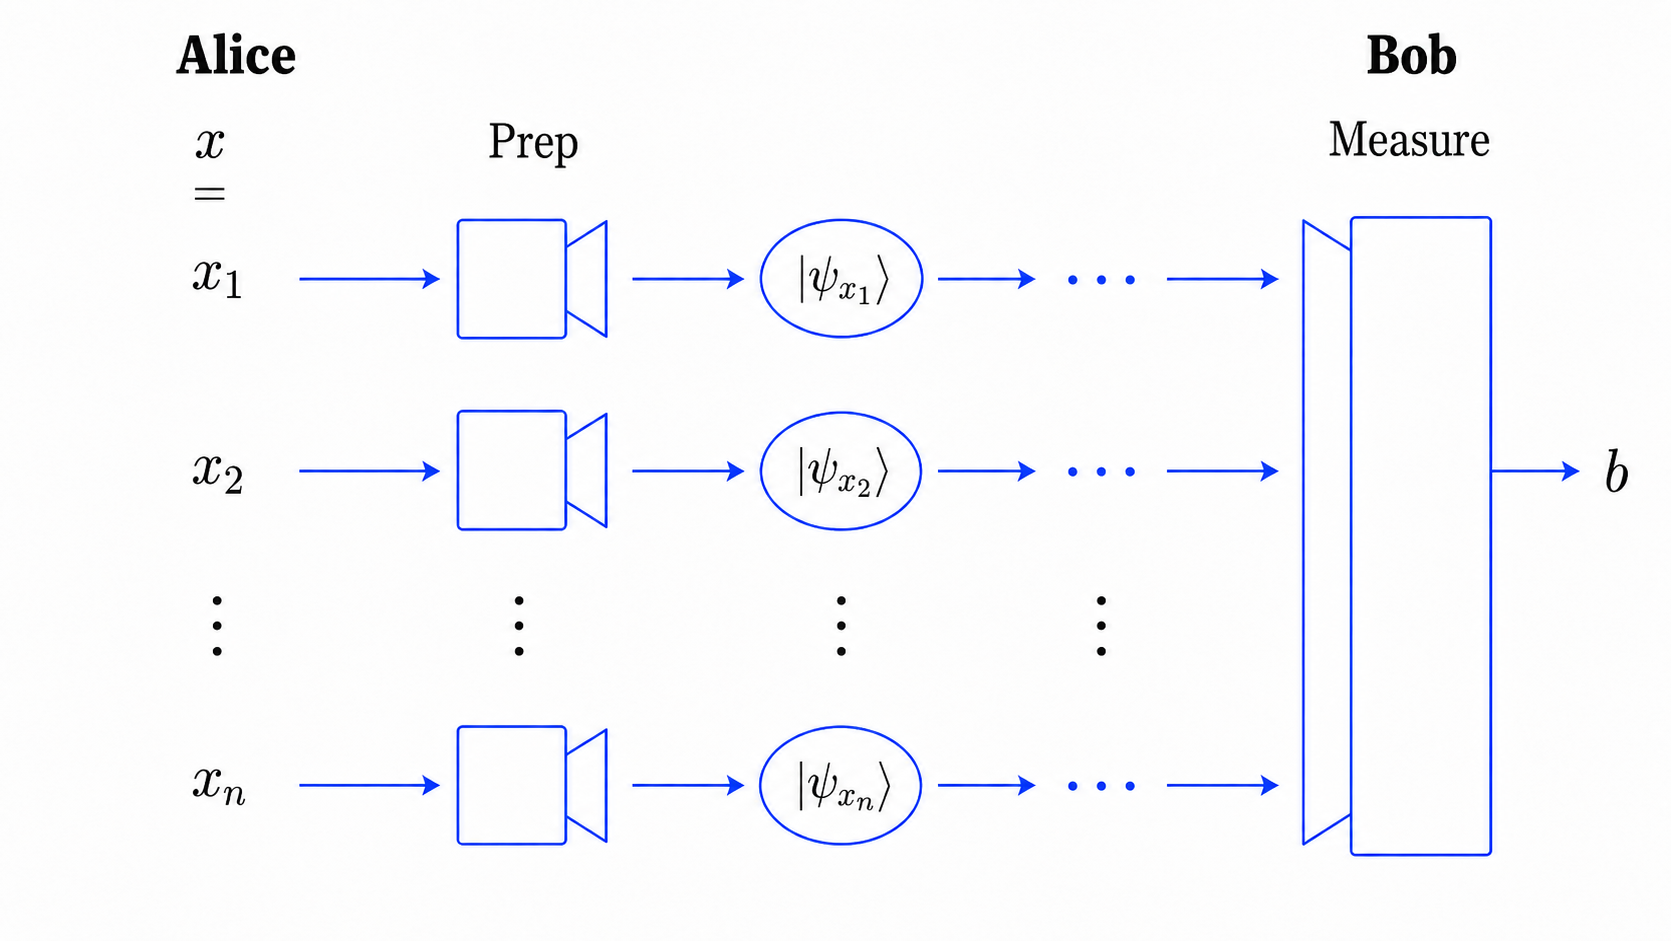
\includegraphics[width=\textwidth]{figs/ch5_qseq/global_startegy.png}
        \caption{Full-memory strategy.}
        \label{fig:global}
    \end{subfigure}
    \hfill
    \begin{subfigure}[b]{0.495\textwidth}
        \centering
        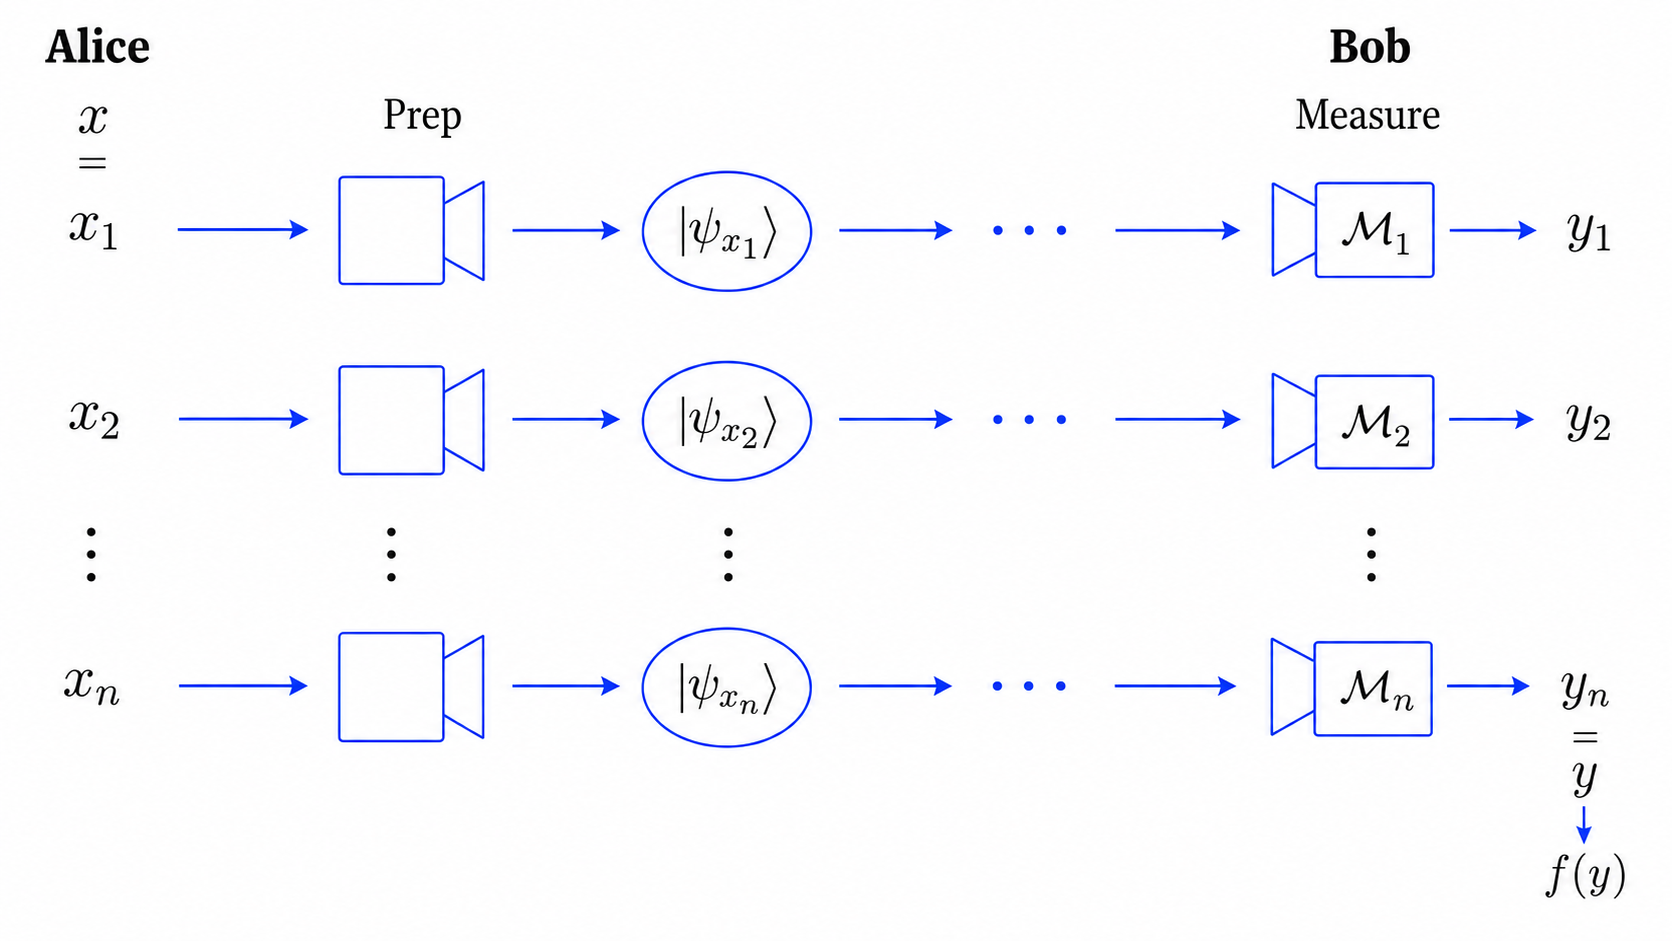
\includegraphics[width=\textwidth]{figs/ch5_qseq/greedy_strategy.png}
        \caption{Memoryless strategy.}
        \label{fig:greedy}
    \end{subfigure}
    \caption{
    Alice prepares the state $\ket{\psi_x} = \ket{\psi_{x_1}} \otimes \ket{\psi_{x_n}}$ and sends it to Bob.
    Bob can either store of all his received states and then perform a joint measurement (Fig.~\ref{fig:global}) or he can measure each off his received states as soon as it is received using predetermined local measurements (Fig.~\ref{fig:greedy}).
    }
    \label{fig:ch1_global_vs_greedy}
\end{figure}

Many information-processing and quantum-computing protocols involve discriminating sequences of quantum states.
The well-known BB84 quantum key distribution scheme is an example where Alice sends Bob qubits chosen at random from the set $\{\ket{0}, \ket{1}, \ket{+}, \ket{-}\}$ \cite{bennett2014quantum}.
From Bob's perspective, the received signal is a quantum sequence whose individual components are drawn from this set.
The central question in such scenarios concerns the resources required to optimally discriminate the given sequence, which might vary significantly across different sequence types.
For example, when discriminating two pure states given a finite number of copies, adaptive local strategies that make limited use of classical memory to condition later measurements based on earlier outcomes achieve the same performance as optimal joint measurements, whereas memoryless strategies generally do so only asymptotically \cite{acin2005multiple}.
However, for two mixed states, joint measurements can strictly outperform all local strategies even in the asymptotic limit \cite{calsamiglia2010local}.
In the quantum change-point detection problem, joint measurements provide an advantage in the minimum-error paradigm \cite{sentis2016quantum}, while for unambiguous detection the optimality of local versus global strategies depends on the overlap between the two states \cite{sentis2017exact}.
For identification of symmetric, pure states, online strategies have been proposed that often achieve optimality using classical memory to store only the last obtained measurement outcome \cite{sentis2022online}.

More recently, for problems where the goal is to identify the entire sequence composed of independently prepared states, it has been shown that memoryless strategies are optimal in the sense that they achieve the same performance as joint measurements, for both minimum-error and unambiguous discrimination \cite{gupta2024unambiguous,gupta2024optimal}.
This observation naturally raises the question of whether such equivalence persists when the discrimination task seeks to learn only specific properties or coarse-grained features of the sequence, rather than its exact identity.

Motivated by this, we initiate a study of learning Boolean properties of quantum sequences.
In a classical information-processing setup, data are represented by bit strings, and computing Boolean functions of these strings, such as the $\XOR$, is elementary; the main challenges lie instead in algorithmic efficiency and robustness of protocols.
In the quantum setting, by contrast, computing even a simple function becomes non-trivial when no classical description of the data is available.
We consider which properties can be optimally learned using memoryless measurement strategies, and which fundamentally require joint measurements across the sequence.
The paradigm we focus on is minimum-error, where the learner might obtain an incorrect value for the property of the sequence and their goal is to minimize this error, and we completely characterize the Boolean functions for which fixed local measurements are optimal.

%%%%%%%%%%%%%%%%%%%%%%%%%%%%%%%%%%%%%%%%%%%%%%%%%%%%%%%%%%%%%%%%%%%%%%%%%%%%%%%%%%%%%%%%%%%%%%%%%%%%%%%%%%%%%%%%%%%%%%%%%%%%%%%%%%%
\section{Background}
%%%%%%%%%%%%%%%%%%%%%%%%%%%%%%%%%%%%%%%%%%%%%%%%%%%%%%%%%%%%%%%%%%%%%%%%%%%%%%%%%%%%%%%%%%%%%%%%%%%%%%%%%%%%%%%%%%%%%%%%%%%%%%%%%%%

In this section, we establish the relevant notations and background for this thesis.
We first review concepts in linear algebra and convex analysis.
Then, we discuss topics in quantum information and semidefinite programming.

\subsection{Notations}

A \emph{complex Euclidean space}, denoted by $\C^n$, is an $n$-dimensional vector space over the field of complex numbers $\C$ equipped with the inner product $\inner{u}{v} = \sum_{i=1}^n \bar{u}_i v_i$ for $u, v \in \C^n$, where $\bar{u}_i$ denotes the complex conjugate of $u_i$.
We will denote complex Euclidean spaces by the letters $\A, \B, \X$ and $\Y$.
We use the shorthand $[n]$ for $\{ 1, \cdots, n \}$.

\subsection{Linear algebra}

The $p$-\emph{norm} for a vector $u \in \C^n$ is defined as
\begin{equation}
    \|u\|_p = \left( \sum_{i=1}^n |u(a)|^p \right)^{\frac{1}{p}}
\end{equation}
for every positive integer $p$ and
\begin{equation}
    \|u\|_\infty = \max \{ |u(a)|\ :\ a \in [n] \}.
\end{equation}

For an operator $A$, we define its \emph{adjoint} as the operator $A^*$ which is computed as $A^* = \overline{A^\top}$ where $A^\top$ is the transpose of $A$ and $\bar{A}$ is the entry-wise conjugate of $A$.

For operators
\begin{equation*}
    A = \begin{pmatrix}
        a_{11} & \cdots & a_{1n} \\
        \vdots & \ddots & \vdots \\
        a_{m1} & \cdots & a_{mn}
    \end{pmatrix} \in \C^{m \times n}
    \quad \text{and} \quad
    B = \begin{pmatrix}
        b_{11} & \cdots & b_{1q} \\
        \vdots & \ddots & \vdots \\
        b_{p1} & \cdots & b_{pq}
    \end{pmatrix} \in \C^{p \times q},
\end{equation*}
we define its \emph{tensor product} as
\begin{equation}
    A \otimes B = \begin{pmatrix}
        A b_{11} & \cdots & A b_{1q} \\
        \vdots & \ddots & \vdots \\
        A b_{p1} & \cdots & A b_{pq}
    \end{pmatrix} \in \C^{mp \times nq}.
\end{equation}

The \emph{trace} of $A \in \C^{n \times n}$ is defined as $\tr(A) = \sum_{i=1}^n A(i, i)$.
The trace function satisfies $\tr(AB) = \tr(BA)$ for all $A \in \C^{m \times n}$ and $B \in C^{m \times p}$.
This is called the \emph{cyclic property} of trace.
This function gives us an inner product as $\inner{A}{B} = \tr(A^* B)$ for all $A \in \C^{m \times n}$ and $B \in C^{m \times p}$.

We denote the largest and smallest eigenvalue of an operator $A$ by $\lambda_{\mathrm{max}}(A)$ and $\lambda_{\mathrm{min}}(A)$ respectively.
An operator $A \in \C^{n \times n}$ is said to be \emph{Hermitian} if it satisfies $A = A^*$.
We denote the set of all Hermitian operators on $\X$ as $\Herm(\X)$.
The eigenvalues of a Hermitian operator are real and thus can be ordered in either the increasing or decreasing order.

An operator $B \in \C^{n \times n}$ is said to be \emph{positive semidefinite} if it admits the decomposition $B = A^* A$ for $A \in \C^{n \times n}$.
The set of all positive semidefinite operators on $\Y$ are denoted as $\Pos(\Y)$.
Every positive semidefinite operator is Hermitian.
The eigenvalues of a positive semidefinite operator are non-negative.
The notation $B \geq 0$ is used to indicate that $B$ is positive semidefinite.
For operators $A, B \in \Herm(\X)$, $A \geq B$ is used to denote that $A-B$ is positive semidefinite.
For a positive semidefinite operator $B$, its \emph{square root} is the operator $B^{1/2}$ satisfying $B^{1/2}\ B^{1/2} = B$.

An operator $X \in \C^{n \times n}$ is \emph{invertible} is there exists an operator $Y \in \C^{n \times n}$ such that $YX = \id$.
When such a $Y$ exists it is denoted by $X^{-1}$.
Since $X$ is square, we also have that $X X^{-1} = \id$.
The \emph{Moore-Penrose pseudoinverse} of $X$ is the operator $X^+$ satisfying:
\begin{enumerate}
    \item $X\ X^+\ X = X$,
    \item $X^+\ X\ X^+ = X^+$, and
    \item $X\ X^+$ and $X^+\ X$ are both Hermitian.
\end{enumerate}

An operator $U \in \C^{n \times n}$ is an \emph{unitary} operator if it preserves the Euclidean norm, i.e., $\|Ux\| = \|x\|$ for all $x \in \C^n$.
These operators preserve inner products as well, i.e., $\inner{Ux}{Uy} = \inner{x}{y}$ for all $x, y \in \C^{n \times n}$.
They satisfy the equation $U^* U = U U^* = \id$ and are invertible.

For an operator $A \in \C^{m \times n}$ and a real number $p \geq 1$, we define the \emph{Schatten $p$-norm} as
\begin{equation}
    \| A \|_p = \left( \Tr((A^* A)^\frac{p}{2}) \right)^\frac{1}{p}
\end{equation}

The Schatten $1$-norm is also referred to as the \emph{trace} norm and the Schatten $2$-norm is referred to as the \emph{Frobenius} norm.

%The Frobenius norm is defined as the norm that this inner product induces, i.e., 
%\begin{equation} 
%\| X \|_F = \sqrt{\tr(X^2)}. 
%\end{equation}
The Cauchy-Schwarz inequality for Hermitian matrices 
\begin{equation} 
|\inner{X}{Y}| \leq \| X \|_F \| Y \|_F 
\end{equation} 
with equality if and only if $X$ and $Y$ are linearly dependent. 
Therefore, if \emph{nonzero} Hermitian $X$ and $Y$ satisfy 
\begin{equation} 
\inner{X}{Y} = \| X \|_F \| Y \|_F 
\end{equation} 
then there must exist $\lambda \neq 0$ such that $X = \lambda Y$.

For complex Euclidean spaces $\A$ and $\B$, the set of all linear mappings from $\A$ to $\B$ is referred to as \emph{linear operators} and is denoted by $L(\A, \B)$.
The shorthand $L(\A)$ is used for $L(\A, \A)$.
The set of all linear mappings from $\mathrm{L}(\A)$ to $\mathrm{L}(\B)$ is denoted by $\mathrm{T}(\A, \B)$.
The \emph{adjoint} of a map $\Phi \in \mathrm{T}(\A, \B)$ is the map $\Phi^* \in \mathrm{T}(\B, \A)$ satisfying $\inner{\Phi^*(A)}{B} = \inner{A}{\Phi(B)}$ for all $A \in \mathrm{L}(\A)$ and $B \in \mathrm{L}(\B)$.
We use the shorthand $T(\A)$ for $T(\A, \A)$.
The \emph{partial trace} map, denoted by $\Tr_\A \in T(\A \otimes \B, \A)$, defined as $\Tr_\A = \Tr \otimes \id_{L(\B)}$.
This satisfies $(\Tr \otimes \id_{L(\B)})(A \otimes B) = \Tr(A) B$ for all $A \in L(\A)$ and $B \in L(\B)$.
We define the map $\Tr_\B \in T(\A \otimes \B, \A)$ similarly.
A map $\Xi \in T(\A, \B)$ is \emph{Hermiticity-preserving} if $\Xi(A) \in \Herm(\B)$ for all $A \in \Herm(\A)$.

The \emph{Gram matrix} $G$ of a set of vectors $\{v_1, \dots, v_N\}$ is a Hermitian positive semidefinite matrix whose entries are given by $G_{ij} = \inner{v_i}{v_j}$.

An $N \times N$ \emph{Toeplitz matrix} $T$ is a matrix with entries satisfying  
\begin{equation}
    T_{i, j} = T_{i + 1, j + 1} \text{ for all } i, j = \{1, \dots, N-1\}.
\end{equation}

This Toeplitz matrix can be written as
\begin{align*}
    T = 
        \begin{pmatrix}
            t_0 & t_{-1} & t_{-2} & \cdots & t_{-(N - 1)} \\
            t_1 & t_0 & t_{-1} & \cdots & t_{-(N - 2)} \\
            t_2 & t_1 & t_0 & \cdots & t_{-(N - 3)} \\
            \vdots & \vdots & \vdots & \ddots & \vdots \\
            t_{N - 1} & t_{N - 2} & t_{N - 3} & \cdots & t_0
        \end{pmatrix},
\end{align*}
noting that every superdiagonal has constant entries.
Since each diagonal of the Toeplitz matrix has the same value, we can alternately express $T$ as
\begin{align}
    \label{eq:Toep_mat}
    T = \sum_{k = -(N-1)}^{N-1} t_k \Theta_{k},
\end{align}
where $\Theta_k$ is an $N \times N$ Toeplitz matrix with ones on the $k$-th diagonal and zeros elsewhere.
Here, $k = 0$ indicates the principal diagonal, $k > 0$ denotes the sub-diagonals, and $k < 0$ corresponds to the super-diagonals.
Note that a Toeplitz matrix is not necessarily square.

A set $\mathcal{C}$ is \emph{convex} if we have $\lambda x + (1 - \lambda) y \in \mathcal{C}$, for all $x, y \in \mathcal{C}$ and $\lambda \in [0, 1]$.
A set $\K$ is a \emph{cone} if $\lambda x \in \K$ for all $x \in \K$ and $\lambda \in [0, 1]$.
A cone that is also convex is referred to as a \emph{convex cone}.
%We say that $\K$ is a convex cone if it is convex and also closed under nonnegative scaling, meaning that if $x \in \K$ then $\lambda x \in \K$ for all $\lambda \geq 0$. 
A cone program is the study of optimizing a linear function over a variable in a convex cone $\K$ subject to affine constraints. 
In standard form, we can write one as 
\begin{equation} 
    \text{maximize } \Big\{ \inner{X}{A} : \Xi(X) = B, \; X \in \K \Big\} 
\end{equation} 
where $\Xi$ is a hermiticity-preserving linear map, and $A$ and $B$ are Hermitian.
The \emph{convex hull} of $\A$, denoted $\conv(\A)$, is the intersection of all convex sets containing $\A$.

An order-$r$ \emph{Krylov subspace} generated by an $n \times n$ matrix $A$ and an $n$-dimensional vector $b$ is the set of vectors
\begin{equation*}
    \K_r(A, b) = \mathrm{span} \left\{ b, A b, A^2 b, \cdots, A^{r-1} b \right\}.
\end{equation*}
Let $r_0 = \dim \mathrm{span} \left\{ b, A b, A^2 b, \cdots \right\}$.
We have that $\left\{ b, A b, A^2 b, \cdots, A^{r-1} b \right\}$ are linearly independent unless $r > r_0$.

\subsection{Quantum information}

A \emph{density} operator is a positive semidefinite operator with unit trace.
We denote the set of all density operators on $\X$ as $\mathrm{D}(\X)$.
We define a \emph{quantum state} as a density operator and commonly refer to this simply as a state.

Consider the set of states $\{\rho_1, \cdots, \rho_n\}$ and an associated set of probabilities $\{p_1, \cdots, p_n\}$.
The set $\{(p_i, \rho_i)\}$ for $i \in [n]$ is referred to as an \emph{ensemble} of states, and the state $\rho = \sum_{i=1}^n p_i \rho_i$ is said to be a \emph{mixture} of these states.
A state with rank one is referred to as a \emph{pure} state.

A state $\rho \in \D(\X)$ is said to be a \emph{product} state if it can be expressed as $\rho = \sigma_1 \otimes \cdots \otimes \sigma_n$ for density matrices $\sigma_1, \cdots, \sigma_n$.
States that cannot be represented as convex combination of such product states are said to be \emph{entangled}.

The \emph{maximally mixed} state in a complex Euclidean space $\X$ is defined as 
\begin{equation}
    \omega_{\mathrm{MM}} = \frac{\id}{\dim(\X)}.
\end{equation}
The state of \emph{uniform superposition} in $\X = \C^n$ is defined as $\omega_{\mathrm{US}} = \kb{\psi}$ where
\begin{equation}
    \ket{\psi} = \frac{1}{\sqrt{n}} \sum_{i=1}^n \ket{i}.
\end{equation}

\emph{Measurements} are a set of positive-operator valued measure (POVM) operators $\{M_i\}$ where each operator $M_i$ is positive semidefinite and $\sum_i M_i = \id$.

\subsection{Tests in quantum computing}\label{sec:QC_bg} 

\paragraph{Swap test.}

Given two (possibly unknown) pure states $\ket{\psi}$ and $\ket{\phi}$, the swap test outputs a Bernoulli random variable that is $0$ with probability $\frac{1}{2} + \frac{1}{2}|\braket{\psi}{\phi}|^2$.
Figure~\ref{fig:inner_product_circuit} (a) depicts the corresponding circuit.
One can learn $|\braket{\psi}{\phi}|^2$ to additive accuracy $\epsilon$ with failure probability at most $\delta$ using $\Ocomp \left(\frac{1}{\epsilon^2} \log \left( \frac{1}{\delta} \right) \right)$ copies of the states and $\tilde{\Ocomp} \left(\frac{1}{\epsilon^2} \log \left( \frac{1}{\delta} \right) \right)$ operations~\cite{buhrman2001quantum,huang2019near}.

\paragraph{Hadamard test.}

Given access to a unitary $U$ that maps the state $\ket{\psi}$ to the state $\ket{\phi}$, this method creates a random variable whose expected value is the real part of $\braket{\psi}{\phi}$.
Figure~\ref{fig:inner_product_circuit} (b) illustrates the circuit for this procedure.
The imaginary part of $\braket{\psi}{\phi}$ can be computed by applying a phase gate $S$ on the first qubit before the controlled unitary operation.
We can learn $|\braket{\psi}{\phi}|^2$ to additive accuracy $\epsilon$ with failure probability at most $\delta$ using $\Ocomp \left(\frac{1}{\epsilon^2} \log \left( \frac{1}{\delta} \right) \right)$ copies of the states and $\tilde{\Ocomp} \left(\frac{1}{\epsilon^2} \log \left( \frac{1}{\delta} \right) \right)$ operations~\cite{aharonov2006polynomial,huang2019near}.

\begin{figure}[ht]
    \centering
    \begin{subfigure}[b]{0.495\textwidth}
        \centering
        \begin{quantikz}
            \lstick{$\ket{0}$} & \gate{H} & \ctrl{2} & \gate{H} & \meter{} & \cw \\
            \lstick{$\ket{\psi}$} & \qw & \swap{1} & \qw & \qw & \qw \\
            \lstick{$\ket{\phi}$} & \qw & \swap{} & \qw & \qw & \qw
        \end{quantikz}    
        \caption{Circuit for swap test.}
    \end{subfigure}
    \hfill
    \begin{subfigure}[b]{0.495\textwidth}
        \centering
        \begin{quantikz}
            \lstick{$\ket{0}$} & \gate{H} & \ctrl{1} & \gate{S^b} & \gate{H} & \meter{} & \cw \\
            \lstick{$\ket{\psi}$} & \qw & \gate{U} & \qw & \qw & \qw & \qw \\
        \end{quantikz}    
        \caption{Circuit for Hadamard test.}
    \end{subfigure}
    \caption{
    Circuits to learn the inner product between two (perhaps unknown) states $\ket{\psi}$ and $\ket{\phi}$.
    The swap test can approximate $|\braket{\psi}{\phi}|$ from many measured samples. 
    When $b = 0$, the Hadamard test approximates from many samples $\Re(\braket{\psi}{\phi})$, and when $b = 1$, $\Im(\braket{\psi}{\phi})$ can be approximated instead.
    The unitary $U$ maps the state $\ket{\psi}$ to the state $\ket{\phi}$. 
    }
    \label{fig:inner_product_circuit} 
\end{figure}

\subsection{Semidefinite programming} \label{ss:ch1_intro-SDP}

Semidefinite programming is an area of convex optimization where the goal is to optimize a linear function of a positive semidefinite matrix $X$ over affine constraints. 
A semidefinite program (SDP) can be written in standard form
    \begin{equation*}    
        \begin{aligned}
            \alpha = \min \quad & \inner{C}{X} \\
            \suchthat \quad & \inner{A_i}{X} = b_i,\ i \in \{1, \dots, m\} \\
            & X \succcurlyeq 0,
        \end{aligned}
    \end{equation*}
where the matrices $C$ and $A_i$ are Hermitian and $b_i$ are real. 
Every SDP has a dual which is an SDP itself and is defined as 
    \begin{equation}
        \label{eq:power_rangers_SPD}
        \begin{aligned}
            \beta = \max \quad & \inner{b}{y} \\
            \suchthat \quad & \sum_{i=1}^m y_i A_i \preccurlyeq C \\
            & y \in \mathbb{R}^m.  
        \end{aligned}
    \end{equation}     
We have that $\alpha \leq \beta$, a fact known as weak duality. 
If both $\alpha$ and $\beta$ are finite and one has a feasible solution where the inequalities are strict (known as strict feasibility), then $\alpha = \beta$. 
This condition is known as strong duality.

The above optimization in this case is called \emph{semidefinite programming} and is of great interest in many areas including combinatorial optimization~\cite{tunccel2016polyhedral} and quantum information~\cite{watrous2018theory} and we refer to a specific instance as a semidefinite program. 
While optimizing over separable operators is indeed intractable, one can often solve SDPs efficiently. 
Current numerical solvers for solving SDPs exist such as CVX~\cite{grant2014cvx}, SeDuMi~\cite{sturm1999using}, SDPT3~\cite{toh1999sdpt3} and Mosek~\cite{andersen2000mosek}. 

Since SDPs can often be solved efficiently, they are a popular choice for approximating convex sets which are difficult to deal with.%, a great example being $\Sep$.